% 2007 年江西卷理科第 8 题：四个形状不同、内空高度与杯口半径相等的圆口酒杯。
%   从左到右：半球形杯、圆锥形杯、圆台形杯、圆柱形杯；虚线表示剩余半杯酒的高度。
% 来源 PDF：gaokaomath-src/普通高考/2007/2007江西理.pdf
% SHA-256：6602cbc393b02e9940beb0035be6e2a28d88a77e0e7792260dcd4c873b542a82
% 原页：2007江西理.pdf 第 1 页（A3 三栏）第 2 栏，书页码 385。
% 重绘依据：按原页四种杯形与半杯液面位置重绘，高度差不按严格比例。
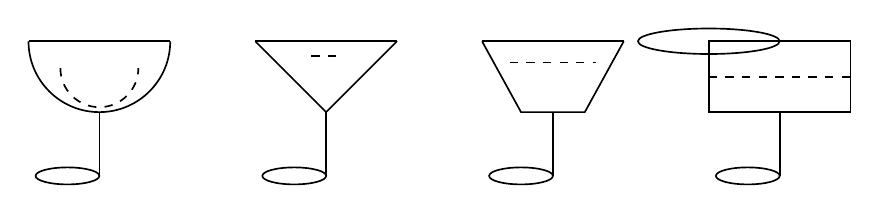
\begin{tikzpicture}[scale=0.9, semithick,
  every node/.style={inner sep=1pt}]

  % ---------------- 半球形杯 ----------------
  \begin{scope}[shift={(0,0)}]
    \draw (-1,3) arc[start angle=180,end angle=360,radius=1];
    \draw (-1,3) -- (-1,3);
    \draw (-1,3) -- (1,3);
    \draw[dashed] (-0.55,2.62) arc[start angle=180,end angle=360,radius=0.55];
    \draw (0,2) -- (0,1.1);
    \draw (-0.45,1.1) ellipse (0.45 and 0.12);
  \end{scope}

  % ---------------- 圆锥形杯 ----------------
  \begin{scope}[shift={(3.2,0)}]
    \draw (-1,3) -- (0,2) -- (1,3);
    \draw (-1,3) -- (1,3);
    \draw[dashed] (-0.21,2.79) -- (0.21,2.79);
    \draw (0,2) -- (0,1.1);
    \draw (-0.45,1.1) ellipse (0.45 and 0.12);
  \end{scope}

  % ---------------- 圆台形杯 ----------------
  \begin{scope}[shift={(6.4,0)}]
    \draw (-1,3) -- (-0.45,2) -- (0.45,2) -- (1,3);
    \draw (-1,3) -- (1,3);
    \draw[dashed] (-0.61,2.7) -- (0.61,2.7);
    \draw (0,2) -- (0,1.1);
    \draw (-0.45,1.1) ellipse (0.45 and 0.12);
  \end{scope}

  % ---------------- 圆柱形杯 ----------------
  \begin{scope}[shift={(9.6,0)}]
    \draw (-1,3) -- (1,3) -- (1,2) -- (-1,2) -- cycle;
    \draw (-1,3) ellipse (1 and 0.18);
    \draw[dashed] (-1,2.5) -- (1,2.5);
    \draw (0,2) -- (0,1.1);
    \draw (-0.45,1.1) ellipse (0.45 and 0.12);
  \end{scope}
\end{tikzpicture}
